\subsection{Общая циркуляция атмосферы и океана. Струйные течения. Муссоны. Центры действия атмосферы. Внетропические циклоны и антициклоны. Блокирующие антициклоны. Фронты. Тропические циклоны, тайфуны/ураганы. Полярные мезоциклоны. Бриз. Смерчи/торнадо.}
Основные причины циркуляции атмосферы и океана:
\begin{enumerate}
\item Бароклинная неустойчивость. Неравномерность распределения солнечной энергии по поверхности Земли $\Rightarrow$ градиент температуры $\Rightarrow$ градиент давления.
\item Эффект вращения Земли.
\end{enumerate}

Совокупность этих причин определяет положение постоянных и сезонных центров действия атмосферы (областей высокого и низкого давления, которые качественно влияют на поведение атмосферных структур).

Схема общей циркуляции атмосферы изображена на рис. $\ref{fig:atm_circ}$ и включает в себя: ячейки Хедли ($0-30^\circ$), ячейки Феррела ($30-60^\circ$) и полярные ячейки ($60-90^\circ$).

\begin{figure}[!ht]
\centering
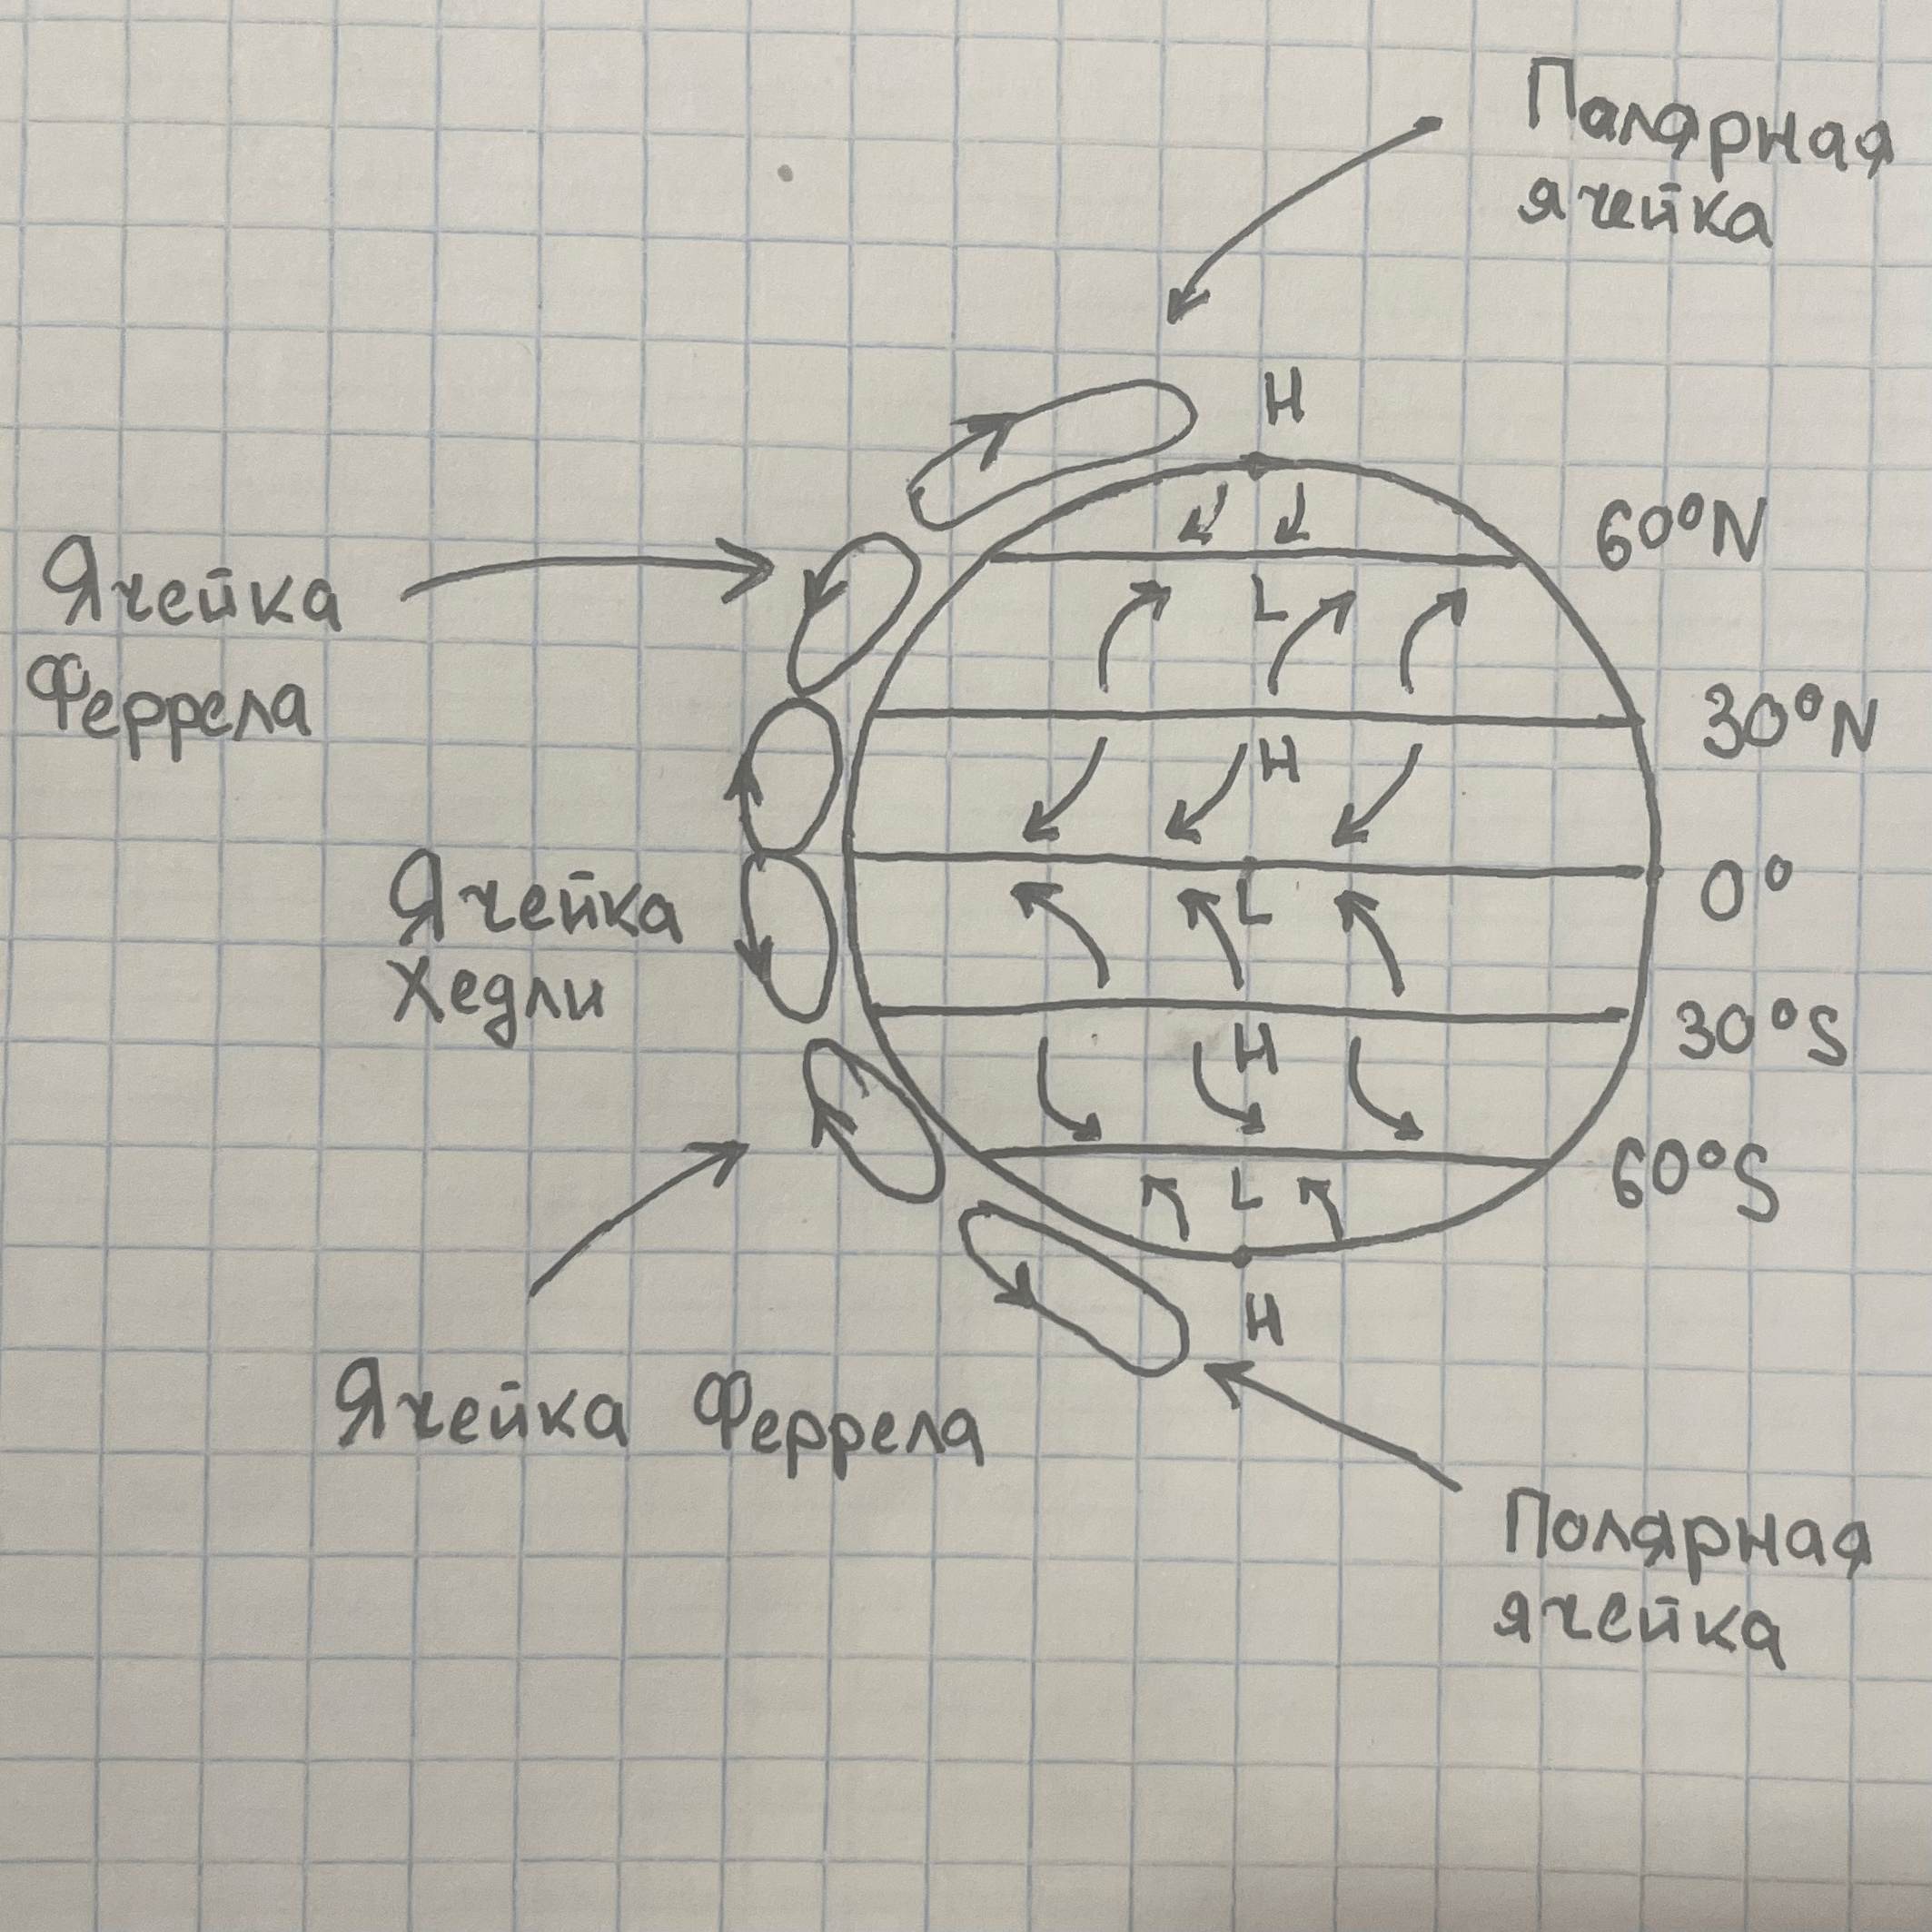
\includegraphics[width=0.4\textwidth]{images/atm_circ.png}
\caption{Схема общей циркуляции атмосферы. $H$ и $L$ -- области высокого и низкого давления, соответственно.}\label{fig:atm_circ}
\end{figure}

Муссон -- ветер на границе материка и океана в зависимости от времени года (лето: океан $\rightarrow$ суша, зима: суша $\rightarrow$ океан).

Бриз -- ветер на границе материка и океана в зависимости от времени суток (день: океан $\rightarrow$ суша, ночь: суша $\rightarrow$ океан).

Пассат -- устойчивый (постоянный) ветер в районе тропиков ($0-30^\circ$), который дует с востока на запад.

Струйные течения -- мощные течения скоростью до 200 м/с в области верхней границы тропосферы (тропопаузы). Положение струйных течений (см. рис. \ref{fig:atm_jets}) совпадает с положением высотных фронтальных зон\footnote{Фронтальная зона -- область с наиболее сильными меридиональными градиентами температуры и давления.}.

\begin{figure}[!ht]
\centering
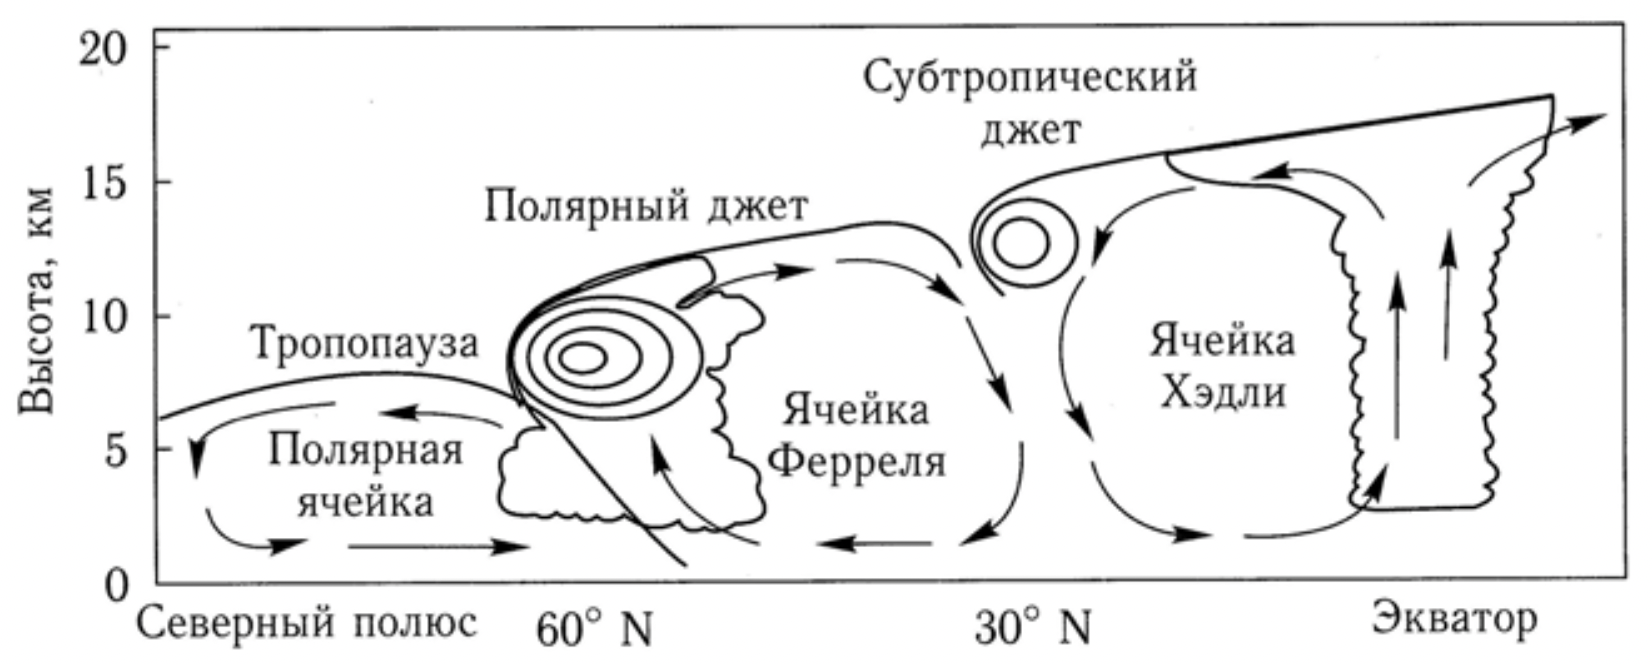
\includegraphics[width=0.5\textwidth]{images/atm_jets.png}
\caption{Расположение струйных течений в меридиональной циркуляции \cite{Переведенцев-Мохов-2013}.}\label{fig:atm_jets}
\end{figure}

Циклон (антициклон) -- атмосферный вихрь\footnote{В северном полушарии направление вращения циклона (антициклона) против (по) часовой стрелки, в южном -- по часовой (против).} синоптического масштаба (размером порядка 1000 км) с пониженным (повышенным) давлением в центре.
Образуется естественным образом из-за силы Кориолиса\footnote{Циклоны и антициклоны не образуются в районе экватора.}.
При прохождении циклона усиливается ветер, облачность и выпадение осадков.
А при прохождении антициклона наоборот -- погода ясная, сухая и малооблачная.

В зависимости от широты циклон может быть тропическим или внетропическим.
Для тропического циклона характерно наличие \textquote{глаза} -- центральной области диаметром 20 -- 30 км с ясной и безветренной погодой.

Тропический циклон, который достиг необычайной силы, в Атлантическом океане называется ураганом, а в Тихом океане -- тайфуном.
Необходимым условием возникновения тропического циклона является достаточный прогрев поверхности океана (не ниже $27^\circ$С).

Блокирующим антициклоном называется высокоустойчивый антициклон, который наблюдается длительное время в области средних широтах и нарушает (блокирует) западный перенос в тропосфере.
Механизмом образования блокирующих антициклонов является обрушение волн Россби в следствие их неустойчивости \cite{Переведенцев-Мохов-2013}.
Существует три типа блокирующих антициклонов: расщепляющий, $\Omega$-блокинг и отсекающий.
Они изображены на рис. \ref{fig:atm_block}.

\begin{figure}[!ht]
\centering
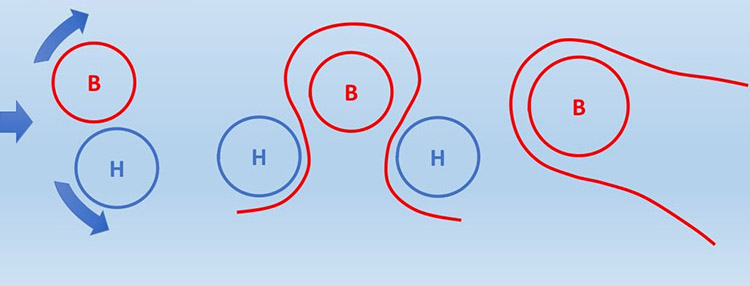
\includegraphics[width=0.5\textwidth]{images/atm_block.jpeg}
\caption{Типы блокирующих антициклонов  (слева направо): расщепляющий, $\Omega$-блокинг (самый частый) и отсекающий (самый редкий).}\label{fig:atm_block}
\end{figure}

Полярный мезоциклон (не путать с полярным вихрем/ячейкой) -- атмосферный вихрь на высоких широтах с размером порядка 100 км, который возникает в результате перемещения холодной воздушной массы над теплой подстилающей поверхностью.

Смерч (торнадо) -- атмосферный вихрь размером порядка 1 км над сушей (океаном) преимущественно с циклоническим направлением вращения.
Обычно образуется из \textquote{материнского} кучево-дождевого облака.

Причины формирования смерчей (торнадо) до конца не изучены, но существуют две основные концепции:
\begin{enumerate}
\item Смерч (торнадо) возникает из-за нисходящих потоков от мезоциклона в суперячейке\footnote{Суперячейка -- мощное кучево-дождевое облако, в структуре которого присутствует мезоциклон.}.
\item Смерч (торнадо) возникает из-за восходящих потоков от завихренности в области влажной и сильно нагретой поверхности.
\end{enumerate}
